\section{Modelos de grano grueso}\label{sec:Ch1CG}

\subsection{Descripciones efectivas}

En nuestro día a día no podemos procesar toda la información de todos los sistemas con los que interactuamos: no nos preocupa la energía cinética individial de cada una de las $10^{23}$ moléculas de agua presente en cada una de las gotas que caen sobre nosotros, sino de qué tan caliente o frío parece el chorro que sale de la llave. Una descripción de \textit{grano grueso} es aquella que no toma en cuenta todas los detalles de un sistema o fenómeno. Dichas particularidades microscópicas pueden omitirse por voluntad del observador (puede que no le sea útil toda la información del sistema, o que la cantidad de información sea demasiado grande como para manjearla) o por simple ignorancia de una porción de los grados de libertad del sistema.

\begin{figure}[ht]
    \centering
    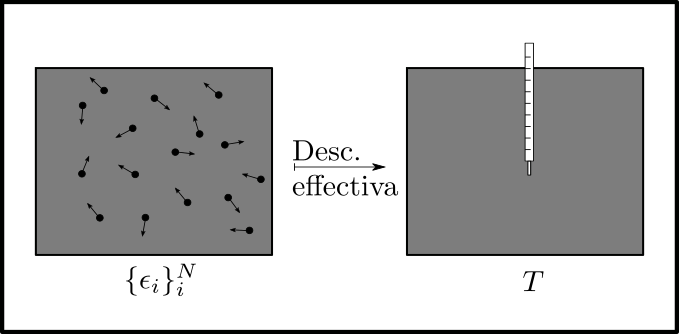
\includegraphics[width=0.6\linewidth]{chapter1/figures/CGT.png}
    \caption{Reducir las energías cinéticas individuales de $N$ partículas a un temperatura es un modelo de grano grueso \ddnote{Tu hiciste esta imagen?}}
    \label{fig:KtoT}
\end{figure}


La termodinámica es un área de la física que trata casi exclusivamente con modelos de grano grueso. Las cantidades termodinámicas: temperatura, presión, volumen, no son sino el resultado de una descripción gruesa de sistemas extremadamente complejos, pues promedian las interacciones y propiedades de $10^{23}$ partículas. En particular, la temperatura de un gas ideal se relaciona con la energía cinética de las particulas de este, a través de la distribución de Boltzman explícitamente a través de un promedio según
\begin{equation}
    T=\frac{1}{k}\frac{2}{3}\expval{E_{\text{cin}}}.
\end{equation}

Cuando se habla de modelos de grano grueso, no se suele hacer referencia a las descripciones efectivas inducidas por la ignorancia. En realidad, cuando se habla de modelos de grano grueso se hace referencia a un modelo impuesto por el observador sobre el sistema. Los modelos de grano grueso que buscan simplificar un problema deshechando información poco útil son comunes en física química \cite{PhysChemI,PhysChemII,PhysChemIII}. El tipo de modelo de grano grueso en el que se centra estre trabajo no es el impuesto por el científico, sino el que proviene de su incapacidad de acceder a toda la información del sistema.

La descripción termodinámica de un sistema de $10^{23}$ partículas corresponde justamente a un modelo de grano grueso inducido por una ignorancia sobre los grados de libertad del sistema. Aún así, auque el observador no cuente con acceso a dicha información, puede deducir que su descripción es meramente efectiva. En efecto, la entropía de un sistema termodinámico es una cantidad que relaciona las coordenadas gruesas con la realidad microscópica.

\subsection{Grano grueso en mecánica cuántica}

En el contexto de la mecánica cuántica, un modelo de grano grueso puede obtenerse trazando sobre un subsistema del sistema de interés. Es importante notar que el subsistema ignorado no es necesariamente una parte que puede ser separada del sistema, como en el caso de dos partículas, sino que puede representar un conjunto de información intrínseca al sistema, pero que se ha decidido ignorar. Por ejemplo, puede que se tome en cuenta el momento angular orbital de una partícula, pero no su espín. De cualquier manera, al subsistema deshechado se le puede llamar \textit{entorno}, y aunque la separación separación sistema - entorno no es siempre posible \cite{Macro-To-Micro}, nos limitamos a los casos en los que los grados de libertad ignorados pueden trazarse a través de la operación de traza parcial, como se discutió en la sección \ref{sec:Ch1PartialTrace}.

Un ejemplo sencillo de un modelo de grano grueso es el de un sistema de dos partículas, del cual únicamente nos importa una. En dicho caso, el modelo puede consistir en estudiar únicamente al operador de densidad reducido correspondiente a la partícula de nuestro interés. De forma fundamental, el modelo de grano grueso consiste en reducir la dimensión del sistema estudiado. En nuestro contexto, una aplicación de grano grueso $\Lambda$ es tal que manda a un operador de densidad $\varrho\in\densityspace{n}$ a algún otro operador de densidad $\rho\in\densityspace{m}$ con $m<n$. Esto es:
\begin{align*}
    \mcF:\densityspace{n}\to \densityspace{m}, n>m
\end{align*}